% ! TeX program = lualatex
\documentclass[a4paper,11pt]{article} 
% packages
\usepackage{censor}
\StopCensoring
\usepackage{fontspec}
\setmainfont{EB Garamond}
% for tironian et fallback
% % \directlua{luaotfload.add_fallback
% % ("emojifallback",
% %      {"Noto Serif:mode=harf"}
% % )}
% % \setmainfont{EB Garamond}[RawFeature={fallback=emojifallback}]

\setmonofont[Scale=MatchLowercase]{Deja Vu Sans Mono}
\usepackage[a4paper,left=2cm,right=2cm,top=\dimexpr15mm+1.5\baselineskip,bottom=2cm]{geometry}
\setlength{\parindent}{0pt}

\usepackage{fancyhdr}       % Headers and footers 
\fancyhead[R]{\normalfont \leftmark}
\fancyhead[L]{}
\pagestyle{fancy}

\usepackage{microtype}      % Slightly tweak font spacing for aesthetics
\usepackage[english]{babel} % Language hyphenation and typographical rules
\usepackage{xcolor}
\definecolor{linkblue}{RGB}{0, 64, 128}
\usepackage[final, colorlinks = false, urlcolor = linkblue]{hyperref} 
% \newcommand{\secref}[1]{\textbf{§~\nameref{#1}}}
\newcommand{\secref}[1]{\textbf{§\ref{#1}~\nameref{#1}}}

\usepackage{mathtools}
\usepackage{changepage}     % adjust margins on the fly

\usepackage{minted}
\usemintedstyle{algol_nu}

\usepackage{pgfplots}
\pgfplotsset{width=\textwidth,compat=1.9}

\usepackage{caption}
\newenvironment{code}{\captionsetup{type=listing}}{}
\captionsetup[listing]{skip=0pt}
\setlength{\abovecaptionskip}{5pt}
\setlength{\belowcaptionskip}{5pt}

\usepackage[yyyymmdd]{datetime}
\renewcommand{\dateseparator}{--}

\usepackage{enumitem}

\usepackage{titlesec}

\author{Andrew Hayes}

\begin{document}
\begin{titlepage}
    \begin{center}
        \hrule
        \vspace*{0.6cm}
        \Huge \textsc{ct420}
        \vspace*{0.6cm}
        \hrule
        \LARGE
       \vspace{0.5cm}
       Real-Time Systems
       \vspace{0.5cm}
       \hrule

       \vfill

       \hrule
        \begin{minipage}{0.495\textwidth} 
            \vspace{0.4em}
            \raggedright
            \normalsize 
            \begin{tabular}{@{}l l}
                Name: & Andrew Hayes \\
                Student ID: & 21321503 \\
                E-mail: & \href{mailto://a.hayes18@universityofgalway.ie}{a.hayes18@universityofgalway.ie} \\
            \end{tabular}
        \end{minipage}
        \begin{minipage}{0.495\textwidth} 
            \raggedleft
            \vspace*{0.8cm}
            \Large
            \today
            \vspace*{0.6cm}
        \end{minipage}
        \medskip\hrule 
    \end{center}
\end{titlepage}

\pagenumbering{roman}
\newpage
\tableofcontents
\newpage
\setcounter{page}{1}
\pagenumbering{arabic}

\section{Introduction}
\subsection{Lecturer Contact Information}
\begin{itemize}
    \item   Name: Dr. Michael Schukat.
    \item   E-mail: \href{mailto://michael.schukat@universityofgalway.ie}{michael.schukat@universityofgalway.ie}.
    \item   Office: CSB-3002.
\end{itemize}

\begin{itemize}
    \item   Name: Dr. Jawad Manzoor.
    \item   E-mail: \href{jawad.manzoor@universityofgalway.ie}{jawad.manzoor@universityofgalway.ie}.
    \item   Office: CSB-3012.
\end{itemize}

\subsection{Assessment}
\begin{itemize}
    \item   2 hours of face-to-face \& virtual labs per week from Week 03.
    \item   30\% Continuous Assessment:
            \begin{itemize}
                \item   2 assignments, 10\% each.
                \item   2 in-class quizzes between Week 07 \& Week 12, worth 5\%.
            \end{itemize}
\end{itemize}

\subsection{Introduction to Real-Time Systems}
A system is said to be \textbf{real-time} if the total correctness of an operation depends not only upon its logical correctness but also upon the time in which it is performed.
Contrast functional requirements (logical correctness) versus non-functional requirements (time constraints).
There are two main categorisation factors:
\begin{itemize}
    \item   \textbf{Criticality:}
            \begin{itemize}
                \item   \textbf{Hard RTS:} deadlines (responsiveness) is critical.
                        Failure to meet these have severe to catastrophic consequences (e.g., injury, damage, death).
                \item   \textbf{Soft RTS:} deadlines are less critical, in many cases significant tolerance can be permitted.
            \end{itemize}

    \item   \textbf{Speed}
            \begin{itemize}
                \item   \textbf{Fast RTS:} responses in microseconds to hundreds of microseconds.
                \item   \textbf{Slow RTS:} responses in the range of seconds to days.
            \end{itemize}
\end{itemize}

A \textbf{safety-critical system (SCS)} or life-critical system is a system whose failure or malfunction may result in death or serious injury to people, loss of equipment / property or severe damage, \& environmental harm.

\section{The Essence of Time: From Measurement to Navigation \& Beyond}
\textbf{Time} is the continued sequence of existence \& events that occurs in an apparently irreversible succession from past, through the present, into the future.
Methods of temporal measurement, or chronometry, take two distinct forms:
\begin{itemize}
    \item   The \textbf{calendar}, a mathematical tool for organising intervals of term;
    \item   The \textbf{clock}, a physical mechanism that counts the passage of time.
\end{itemize}

Global (maritime) exploration requires exact maritime navigation, i.e., longitude \& latitude calculation.
\textbf{Latitude} (north-south) orientation is straightforward; \textbf{longitude} (east-west orientation) requires a robust (maritime) clock.
\\\\
\textbf{Ground-based navigation systems} like LORAN (LOng RAnge Navigation) were developed in the 1940s and were in use until recently, and required fixed terrestrial longwave radio transmitters, and receivers on-board of ships \& planes.
They are also referred to as hyperbolic navigation or multilateration.
The principles of ground-based navigation systems is as follows:
\begin{enumerate}
    \item   A \textbf{master} with a known location broadcasts a radio pulse.
    \item   Multiple \textbf{slave} stations with a known distance from the master send their own pulse, upon receiving the master pulse.
    \item   A \textbf{receiver} receives master \& slave pulses and measures the delay between them.
    \item   This allows the receiver to deduce the distance to each of the stations, providing a fix.
\end{enumerate}

NEED TO FINISH

\section{Time Synchronisation in Distributed Systems}
A \textbf{distributed system (DS)} is a type of networked system wherein multiple computers (nodes) work together to perform a task.
Such systems may or may not be connected to the Internet.
Time \& synchronisation are important issues here: think of error logs in distributed systems -- how can error events recorded in different computers be correlated with each other if there is no common time base?
The problem is that GNSS-based time synchronisation may or may not be available, as GPS signals are absorbed or weakened by building structures.
There is no other time reference such systems can rely on because in such a distributed system there are just a series of imperfect computer clocks.
\\\\
In distributed systems, all the different nodes are supposed to have the same notion of time, but quartz oscillators oscillate at slightly different frequencies.
Hence, clocks tick at different rates (called \textit{clock skew}), resulting in an increasing gap in perceived time.
The difference between two clocks at a given pot is called \textit{clock offset}.
The \textbf{clock synchronisation problem} aims to minimise the clock skew and subsequently the offset between two or more clocks.
A clock can show a positive or negative offset with regard to a reference clock (e.g., UTC), and will need to be resynchronised periodically.
One cannot just set the clock to the ``correct'' time: jumps, particularly backwards, can confuse software and operating systems.
Instead, we aim for gradual compensation by correcting the skew: if a clock runs too fast, make it run slower until correct and if a clock runs too slow, make it run faster until correct.
\\\\
Synchronisation can take place in different forms:
\begin{itemize}
    \item   Based on \textbf{physical} clocks: absolute to each other by synchronising to an accurate time source (e.g., UTC), absolute to each other by synchronising to locally agreed time (i.e., no link to a global time reference), where the term \textit{absolute} means that the differences in timestamps are proper time intervals.

    \item   Based on \textbf{logical} clocks (i.e., clocks are more like counters): timestamps may be ordered but with no notion of measurable time intervals.
\end{itemize}

In either case, the DS endpoints synchronise using a shared network.
For physical clock synchronisation, network latencies must be considered as packets traverse from a sending node to a receiving node.
In a \textbf{perfect network}, messages \textit{always} arrive, with a propagation delay of \textit{exactly} $d$;
the sender sends time $T$ in a message, the receiver sets its clock to $T + d$, and synchronisation is exact.
\\\\
In a \textbf{deterministic network}, messages arrive with a propagation delay $0 < d \leq D$;
the sender sends time $T$ in a message, the receiver sets its clock to $T + \frac{D}{2}$, and therefore the synchronisation error is at most $\frac{D}{2}$.
\textbf{Deterministic communication} is the ability of a network to guarantee that a message will be transmitted in a specified, predictable period of time.  

\subsection{Synchronisation in the Real World}
Most off-the-shelf networks are \textit{asynchronous}, that is, data is transmitted intermittently on a best-effort basis.
They are designed for flexibility, not determinism, and as a result, propagation delays are arbitrary and sometimes even unsymmetric (i.e., upstream \& downstream latencies are different).
Therefore, synchronisation algorithms are needed to accommodate these limitations.

\subsubsection{Cristian's Algorithm}
\textbf{Cristian's algorithm} attempts to compensate for symmetric network delays:
\begin{enumerate}
    \item   The client remembers the local time $T_0$ just before sending a request.
    \item   The server receives the request, determines $T_S$, and sends it as a reply.
    \item   When the client receives the reply, it notes the local arrival time $T_1$.
    \item   The correct time is then approximately $(T_S + \frac{(T_1 - T_0)}{2} )$.
\end{enumerate}

The algorithm assumes symmetric network latency.
If the server is synced to UTC< all clients will follow UTC.
Limitations of Cristian's algorithm include:
\begin{itemize}
    \item   Assumes a symmetric network latency;
    \item   Assumes that timestamps can be taken as the packet hits the wire / arrives at the client;
    \item   Assumes that $T_S$ is right in the middle of the server process; for example, consider the server process being pre-empted just before it sends the response back to the client, which will corrupt the synchronisation of the client.
\end{itemize}

\subsubsection{Berkeley Algorithm}
In the \textbf{Berkeley algorithm}, there is no accurate time server: instead, a set of client clocks is synchronised to their average time.
The assumption is that offsets / skews of all clocks follow some symmetric distribution (e.g., a normal distribution) with some clocks going faster and others slower, and therefore a mean value close to 0.
\begin{enumerate}
    \item   One node is designated to be the \textbf{master node} $M$.
    \item   The master node periodically queries all other clients for their local time.
    \item   Each client returns a timestamp or their clock offset to the master.
    \item   Cristian's algorithm is used to determine and compensate for RTTs, which can be different for each client.
    \item   Using these, the master computes the average time (thereby ignoring outliers), calculates the difference to all timestamps it has received, and sends an adjustment to each client.
            Again, each computer gradually adjusts its local clock.
\end{enumerate}

Client clocks are adjusted to run faster or slower, to be synced to an overall agreed system time.
The client networks is an intranet, i.e., an isolated system.
Therefore, the Berkeley algorithm is an \textbf{internal clock synchronisation algorithm}.
The Berkeley algorithm was implemented in the TEMPO time synchronisation protocol, which was part of the Berkelely UNIX 4.3BSD system.

\subsection{Logical Clocks}
\textbf{Logical clocks} are another concept linked to internal clock synchronisation.
Logical clocks only care about their internal consistency, but not about absolute (UTC) time;
subsequently, they do not need clock synchronisation and take into account the order in which events occur rather than the time at which they occurred.
In practice, if clients or processes only care that event $a$ happens before event $b$, but don't care about the exact time difference, they can make use of a logical clock.
\\\\
We can define the \textbf{happens-before relation} $a \rightarrow b$:
\begin{itemize}
    \item   If events $a$ and $b$ are within the same process, then $a \rightarrow b$ if $a$ occurs with an earlier local timestamp: \textbf{process order}.
    \item   If $a$ is the event of a message being sent by one process, and $b$ is the event of the message being received by another process, then $a \rightarrow b$: \textbf{causal order}.
    \item   We also have \textbf{transitivity:} if $a \rightarrow b$ and $b \rightarrow c$, then $a \rightarrow c$.
\end{itemize}
Note that this only provides a \textit{partial order}:
if two events $a$ and $b$ happen in different processes that do not exchange messages (not even indirectly), then neither $a \rightarrow b$ nor $b \rightarrow a$ is true.
In this situation, we say that $a$ and $b$ are \textbf{concurrent} and write $a \sim b$, i.e., nothing can be said about when the events happened or which event happened first.
\\\\
Happens-before can be implemented using the \textbf{Lamport scheme:}
\begin{enumerate}
    \item   Each process $P_i$ has a logical clock $L_i$, where $L_i$ can be simply an integer variable initialised to 0.
    \item   $L_i$ is incremented on every local event $e$; we write $L_i(e)$ or $L(e)$ as the timestamp of $e$.
    \item   When $P_i$ sends a message, it increments $L_i$ and copies its content into the packet.
    \item   When $P_i$ receives a message from $P_k$, it extracts $L_k$ and sets $L := \text{max}(L_i, L_k)$ and then increments $L_i$.
\end{enumerate}

This guarantees that if $a \rightarrow b$, then $L_i(a) < L_k(b)$, but nothing else.
\\\\
The primary limitation of Lamport clocks is that they do not capture \textbf{causality}.
Lamport's logical clocks lead to a situation where all events in a distributed system are ordered, so that if an event $a$ (linked to $P_i$) ``happened before''  event $b$ (linked to $P_k$), i.e., $a \rightarrow b$, then $a$will allso be positioned in that ordering before $b$ such that $L_i(a) < L_k(b)$ or simply $L(a) < L(b)$;
however, nothing can be said about the relationship between two events $a$ \& $b$ by merely comparing their time values $L_i(a)$ and $L_k(b$.): we can't tell if $a \rightarrow b$ or $b \rightarrow a$ or $a \sim b$ unless they occur in the same process.

\subsubsection{Vector Clocks}
In practice, causality is captured by means of \textbf{vector clocks}:
\begin{enumerate}
    \item   There is an ordered list of logical clocks, with one per process.
            Each process $P_i$ maintains a vector $\vec{V_i}$, initially containing all zeroes.
            Each index $k$ of a vector clock $\vec{V_i}[k]$ represents the number of events that process $P_i$ knows have occurred in process $P_k$.
            $\vec{V_i}[i]$  is the count of events that have occurred locally at process $P_i$, while $\vec{V_i}[k]$ (for $k\neq i$) is the count of events in process $P_k$ that $P_i$ is aware of.

    \item   On a local event $e$, $P_i$ increments its own clock component $\vec{V_i}[i]$.
            If the event is ``message send'', a new $\vec{V_i}$ is copied into the packet, so that on message sends the current vector state is included in the message.

    \item   If $P_i$ receives a message from $P_m$, then each index $\vec{V_i}[k]$ where $k \neq i$ is set to $\text{max}(\vec{V_m}[k], \vec{V_i}[k])$, and $\vec{V_i}[i]$ is incremented.
\end{enumerate}

Intuitively, $\vec{V_i}[k]$is the number of events in process $P_k$ that have been observed by $P_i$.

\begin{figure}[H]
    \centering
    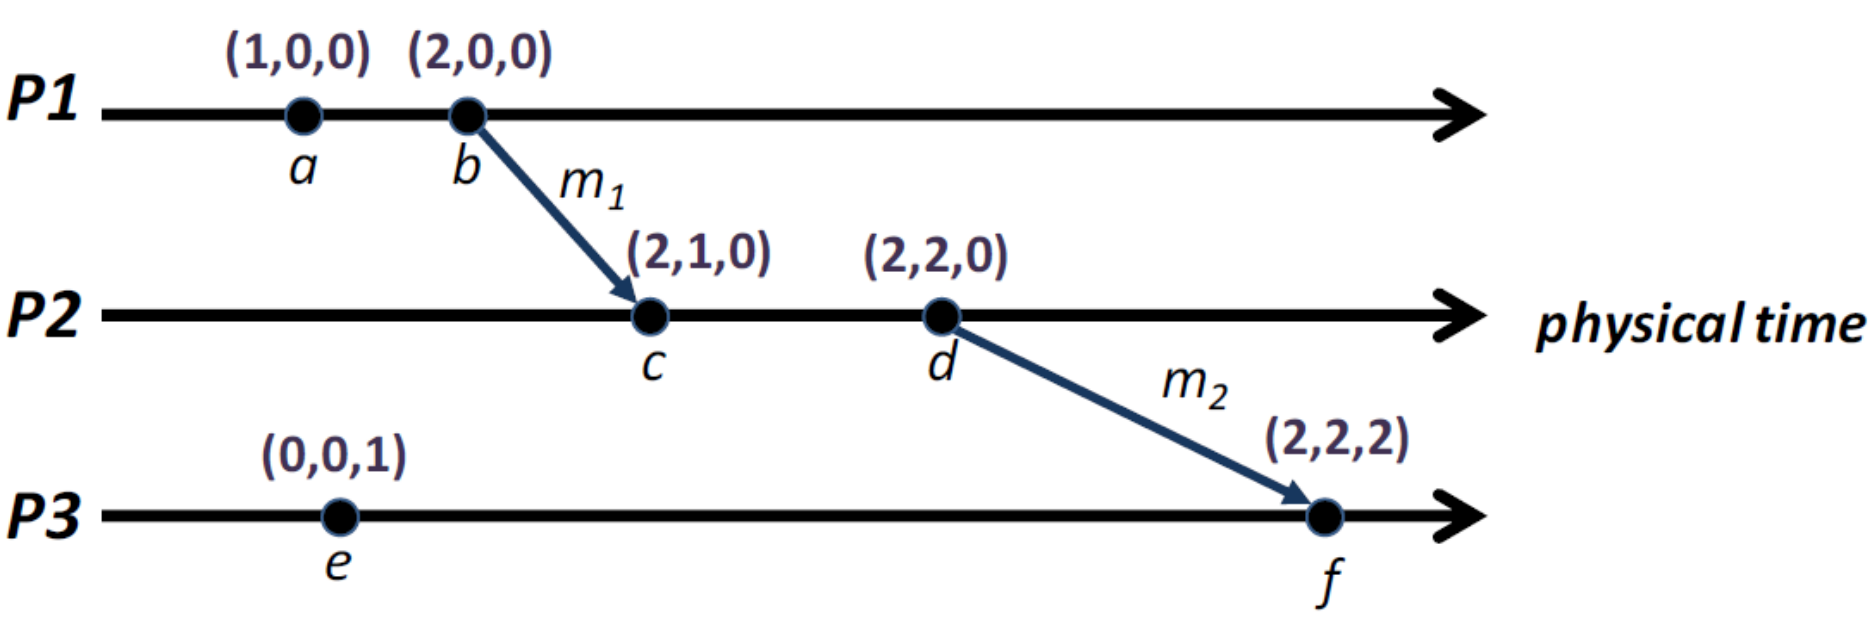
\includegraphics[width=\textwidth]{./images/vector_clocks_example.png}
    \caption{Vector clocks example}
\end{figure}

In the above example, when process $P_2$ receives message $m_1$, it merges the entries from $P_1$'s clock by choosing the maximum value of each position.
Similarly, when $P_3$ receives $m_2$, it merges in $P_2$'s clock, thus incorporating the changes from $P_1$ that $P_2$ already saw. 
Vector clocks explicitly track the transitive causal order: $f$'s timestamp captures the history of $a$, $b$, $c$, \& $d$.
\\\\
To use vector clocks for ordering, we can compare them piecewise:
\begin{itemize}
    \item   We say $\vec{V_i} = \vec{V_j}$ if and only if $\vec{V_i}[k] = \vec{V_j}[k] \forall k$.
    \item   We say $\vec{V_i} \leq \vec{V_j}$ if and only if $\vec{V_i}[k] \leq \vec{V_j}[k] \forall k$.
    \item   We say $\vec{V_i} < \vec{V_j}$ if and only if $\vec{V_i} \leq \vec{V_j}$ and $\vec{V_i} \neq \vec{V_j}$.
    \item   We say $\vec{V_i} \sim \vec{V_j}$ otherwise, e.g., $\vec{V_i} = [2,0,0]$ and $\vec{V_j} = [0,0,1]$.
\end{itemize}

For any two event timestamps $T(a)$ \& $T(b)$:
\begin{itemize}
    \item   if $a \rightarrow b$, then $T(a) < T(b)$; \textbf{and}
    \item   if $T(a) < T(b)$, then $a \rightarrow b$.
\end{itemize}

Hence, we can use timestamps to determine if there is a causal ordering between any two events.

\begin{figure}[H]
    \centering
    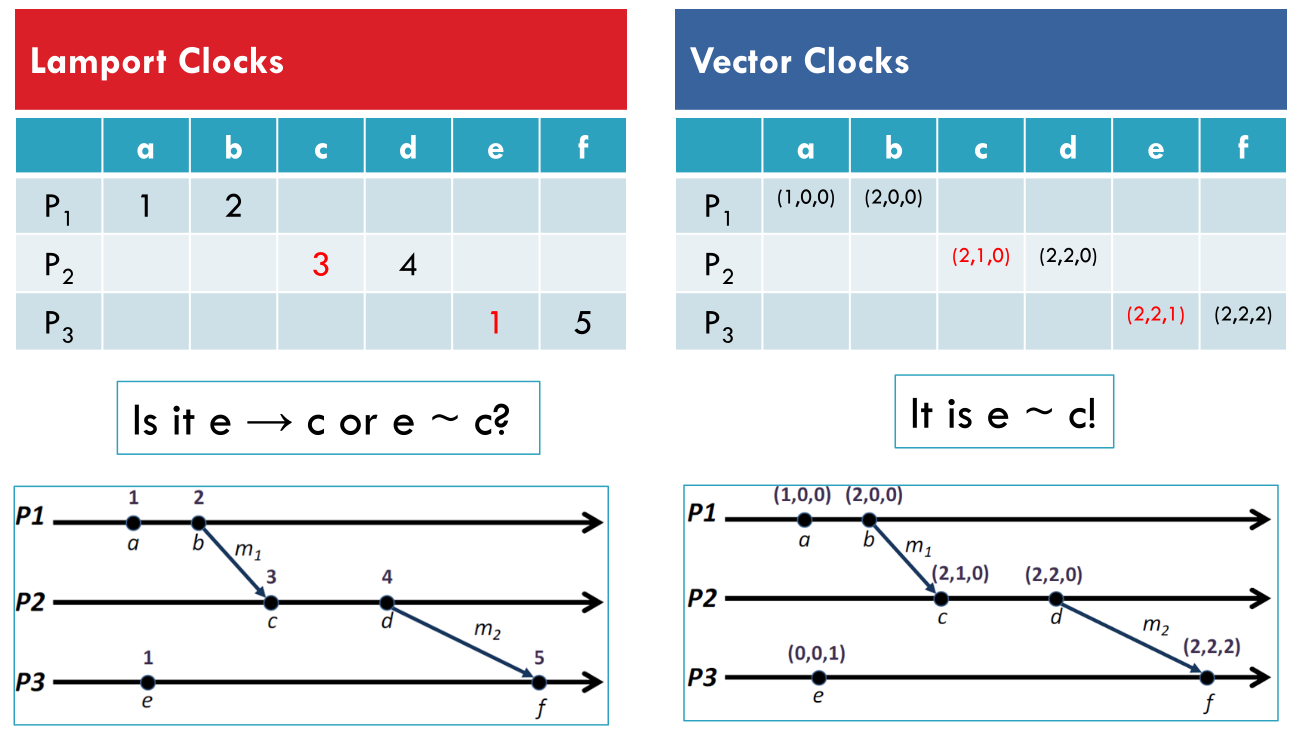
\includegraphics[width=\textwidth]{./images/vector_vs_lamport.png}
    \caption{Lamport clocks versus vector clocks}
\end{figure}

\section{The NTP Protocol}
The options for computer clocks are essentially as follows:
\begin{itemize}
    \item   \textbf{Option A:} stick to crystals.
            \begin{itemize}
                \item   Costly precision manufacturing.
                \item   Works indoors.
                \item   Temperature Compensated Crystal Oscillator (TCXO).
                \item   Oven Controlled Crystal Oscillator (OCXO).
            \end{itemize}

    \item   \textbf{Option B:} buy an atomic clock (\$50,000 -- \$100,000) or a GNSS receiver (based on an atomic clock, but doesn't work indoors), or a time signal radio receiver if you are based in central Europe.

    \item   \textbf{Option C:} use software-based approaches to discipline cheap crystal clocks.
            Less quality, but useful for certain applications, and works indoors.
\end{itemize}

\textbf{Distributed master clocks} provide a time reference to hosts that are inter-connected via a network.
The underlying time-synchronisation protocols combine aspects of Cristian's algorithm (i.e., RTD calculation) and Berkeley's algorithm (i.e., combining multiple reference time sources).
Good time synchronisation requires:
\begin{itemize}
    \item   Good time references: easily done with GPS, atomic clocks, etc.
    \item   Predictable / symmetric / deterministic network latencies: doable in LAN setups, but not guaranteed in Internet data communication.
\end{itemize}

There are two main distributed master clock protocols:
\begin{itemize}
    \item   \textbf{Network Time Protocol (NTP):} defined in RFC 5905, originally used in the Unix-based NTP daemon, one of the first Internet protocols that ever evolved.
    \item   \textbf{Precision Time Protocol (PTP):} designed for managed networks, e.g., LAN.
\end{itemize}

\begin{figure}[H]
    \centering
    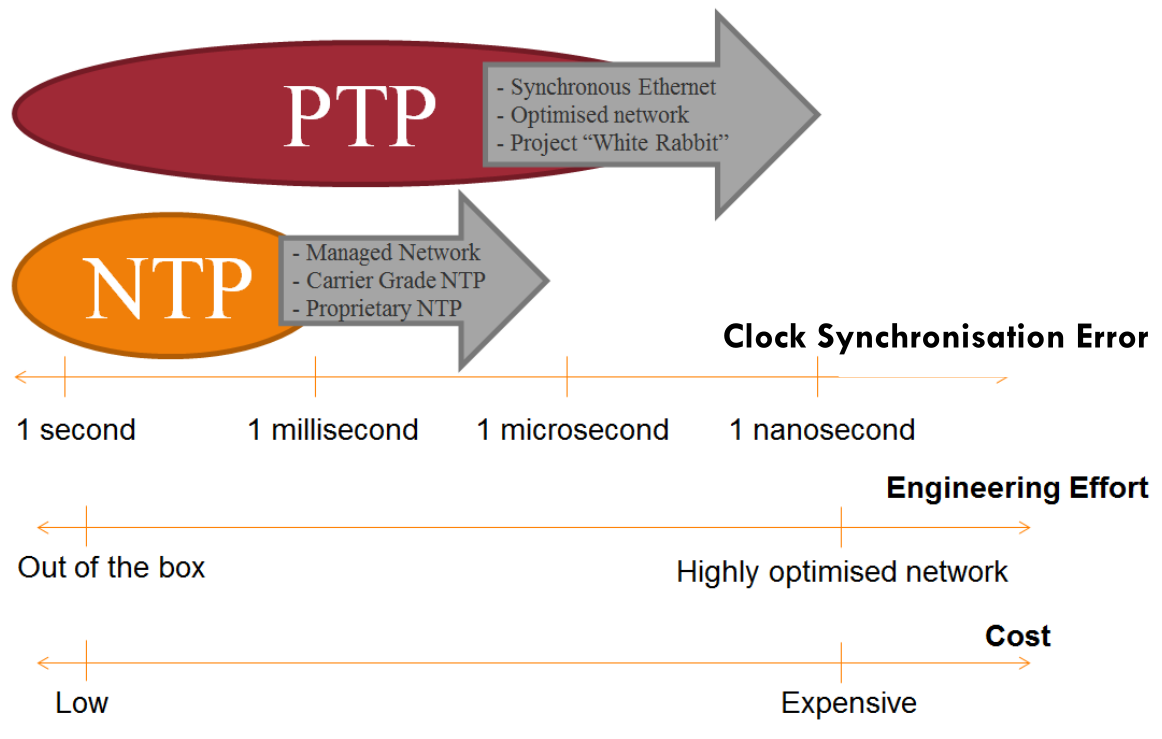
\includegraphics[width=0.7\textwidth]{./images/ntpvsptp.png}
    \caption{NTP \& PTP characteristics}
\end{figure}

In \textbf{uni-directional synchronisation} a reference clock sends a timestamp to a host via a network.
The host then uses the timestamp to set its local clock.
Useful when message latencies are minor relative to the synchronisation levels required.
\\\\
In \textbf{round-trip synchronisation (RTS)} a host sends a request message, receives a reference clock response message with known (local) submission \& arrival times, allowing for the calculation of the round-trip delay (1) and the host clock error (2), i.e., the phase offset.
Variations of RTS form the basis for NTP \& PTP.

\begin{align}
    \delta = (T_{i+3} - T_i) - (T_{i+2} - T_{i+1})
\end{align}
\begin{align}
    \theta = (T_{i+1}-T_i) + \frac{(T_{i+2}-T_{i+3})}{2}
\end{align}

\begin{figure}[H]
    \centering
    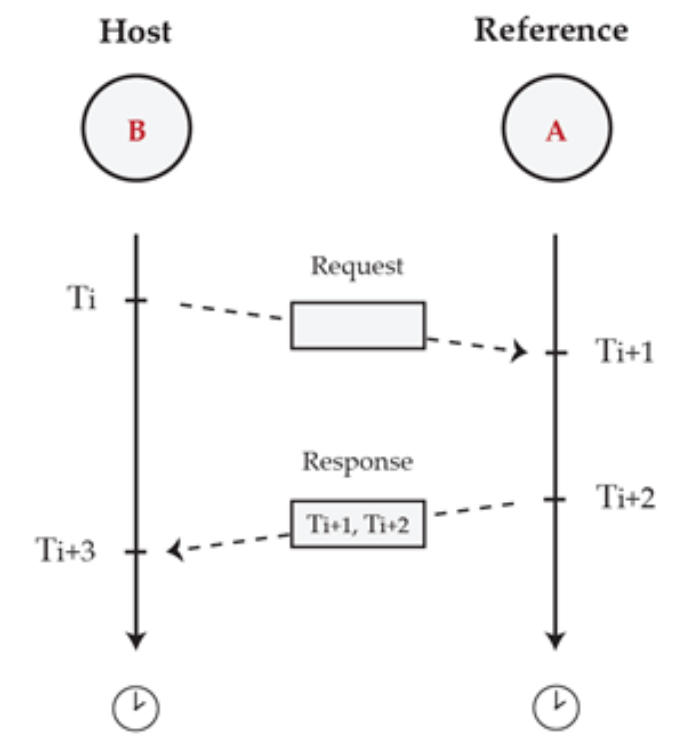
\includegraphics[width=0.4\textwidth]{./images/rts.png}
    \caption{ RTS example }
\end{figure}

\subsection{NTP}
The NTP architecture, protocol, \& algorithms have evolved over the last 40 years to the latest NTP Version 4.
NTP is the standard Internet protocol for time synchronisation \& co-ordinated UTC time distribution.
It is a fault-tolerant protocol, as it automatically selects the best of several available time sources to synchronise with.
It is highly scalable, as the nodes form a hierarchical structure with reference clock(s) at the top:
\begin{itemize}
    \item   Stratum 0: Time Reference Source (e.g., GPS, TAI atomic clocks, DCF 77).
    \item   Stratum 1: Primary Time Server.
\end{itemize}

NTP applies some general aforementioned principles such as avoiding setting clocks backwards and avoiding large step changes;
the required change (positive or negative) is amortised over a series of short intervals (e.g., over multiple ticks).
\\\\
NTP is the longest-running and continuously operating Internet protocol (since around 1979).
Government agencies in many other countries and on all continents (including Antarctica) operate public NTP primary servers.
National \& regional service providers operate public NTP secondary servers synchronised to the primary servers.
Many government agencies, private \& public institutions including universities, broadcasters, financial institutions, \& corporations operate their own NTP networks. 
\begin{figure}[H]
    \centering
    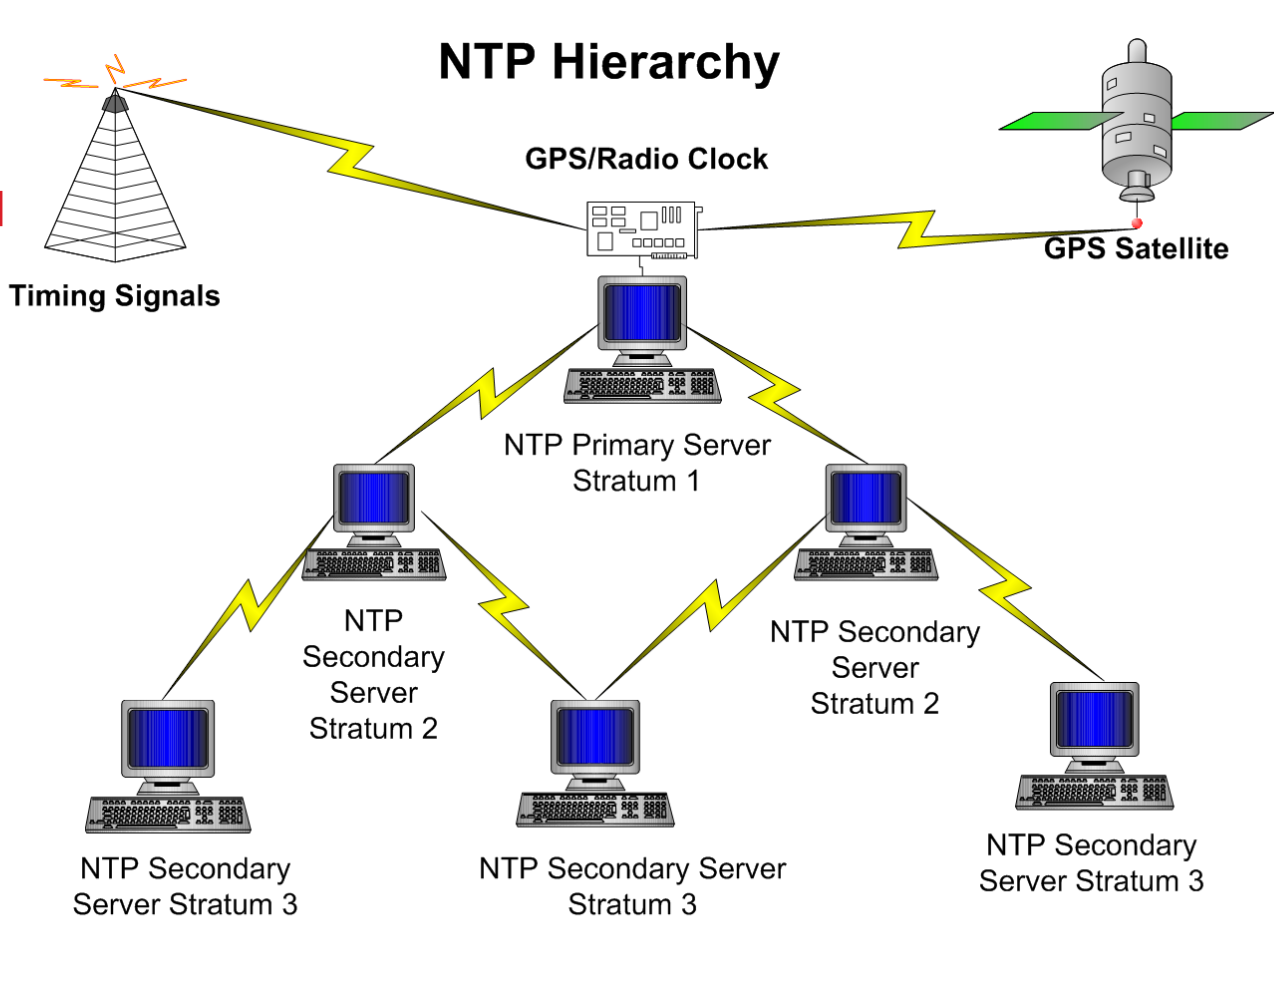
\includegraphics[width=0.5\textwidth]{./images/ntphierarchy.png}
    \caption{ NTP hierarchy }
\end{figure}

In \textbf{client/server mode}, UDP is used for data transfer (no TCP), i.e., NTP over UDP on UDP port 123.
There is also the optional use of broadcasting or multicasting (not covered here).
Several packet exchanges between the NTP client and the Stratum server take place to determine the client offset:
\begin{enumerate}
    \item   The client sends a packet with \textbf{originate timestamp} $A$.
    \item   The server receives the packet and returns a response containing the originate timestamp $A$ as well as the \textbf{receive timestamp} $B$ and the \textbf{transmit timestamp} $C$.
    \item   The client receives this packet and processes $A$, $B$, $C$, as well as the packet arrival time $D$ of the received packet; it then determines the offset and the round-trip delay (RTD).
\end{enumerate}

\begin{figure}[H]
    \centering
    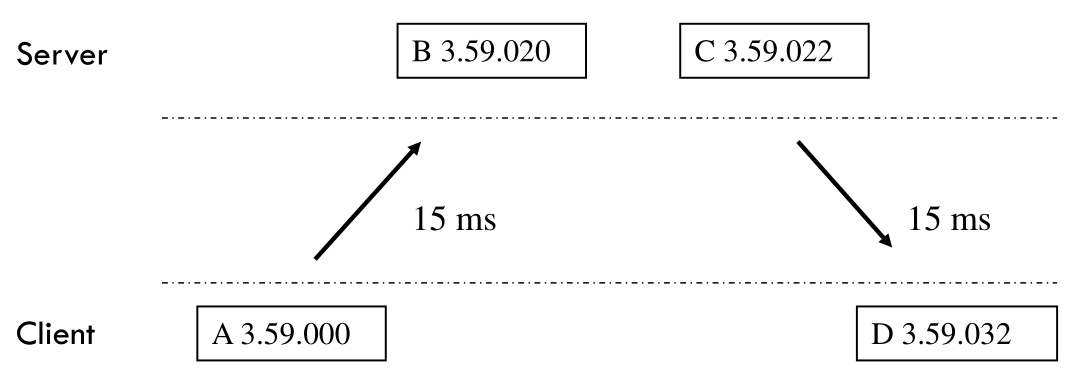
\includegraphics[width=0.7\textwidth]{./images/ntpoperation.png}
    \caption{ NTP operation }
\end{figure}

The above example is of a symmetric network with a 15ms delay each way; the client's clock lags 5ms behind the server's clock:
\begin{align*}
    \text{RTD}      = (D-A)-(C-B) = 32-2 =& 30\text{ms} \\
    \text{Offset}   = \frac{((B-A)+(C-D))}{2} = \frac{(20 + (-10))}{2} =& 5\text{ms}
\end{align*}

\begin{figure}[H]
    \centering
    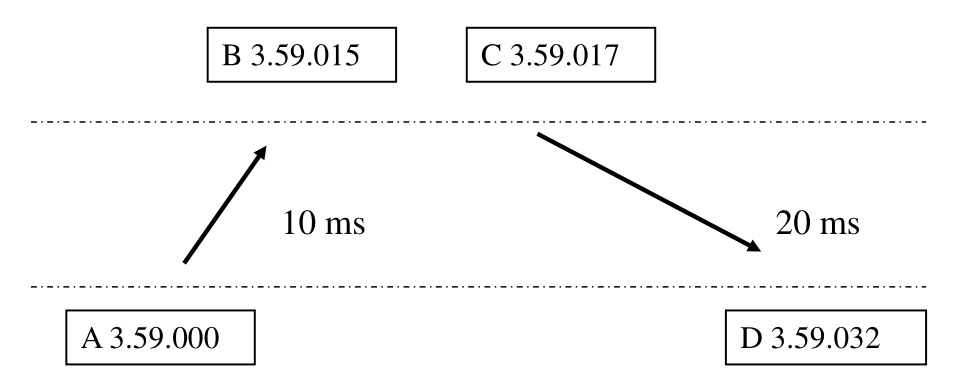
\includegraphics[width=0.7\textwidth]{./images/networkdelayasymmetry.png}
    \caption{ Network delay asymmetry }
\end{figure}

In the above example, the client's clock still lags 5ms behind the servers clock, but there is an asymmetric network latency: 10ms versus 20ms:
\begin{align*}
    \text{RTD}      = (D-A)-(C-B) = 32-2                                =& 30\text{ms} \\
    \text{Offset}   = \frac{((B-A)+(C-D))}{2} = \frac{(15 + (-15))}{2}  =& 0\text{ms}
\end{align*}

Typical NTP performance for various set-ups is as follows:
\begin{itemize}
    \item   Small LAN: \sim10 microseconds best possible case on a 2-node LAN, \sim220 microseconds on a real-world small LAN.
    \item   Typical large-building LAN: \sim2ms.
    \item   Internet with a few hops: 10–20ms.
    \item   Long distance and/or slow or busy link: 100ms–1s.
\end{itemize}

Accuracy is further degraded on networks with asymmetric traffic delays.
\\\\
The \textbf{NTP time format} has a reference scale of UTC.
Time parameters are 64 bits long:
\begin{itemize}
    \item   Seconds since January 1, 1900 (32 bits, unsigned).
    \item   Fraction of second (32 bits, unsigned).
\end{itemize}
The NTP time format has a dynamic range of 136+ years, with rollover in 2036.
Its resolution is 2\textsuperscript{-32} seconds \sim232 picoseconds.

\subsubsection{NTP Protocol Header}
\begin{figure}[H]
    \centering
    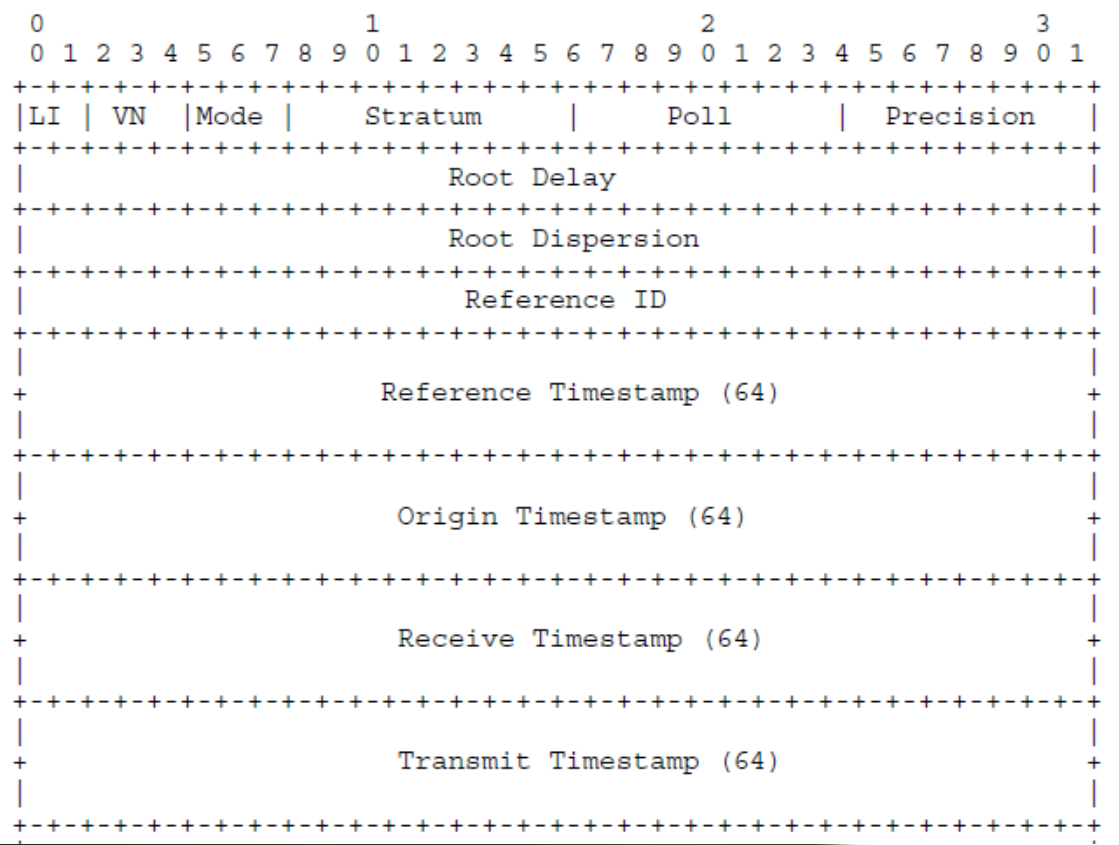
\includegraphics[width=0.7\textwidth]{./images/ntpheader.png}
    \caption{ NTP protocol header }
\end{figure}
\begin{itemize}
    \item   \verb|LI| (\textbf{Leap Indicator}) 2-bit:
            \begin{itemize}
                \item   \verb|0|: no warning;
                \item   \verb|1|: last minute of the day has 61 seconds;
                \item   \verb|2|: last minute of the day has 59 seconds.
            \end{itemize}


    \item   \verb|VN| (\textbf{Version Number}) 2-bit: currently 4. 

    \item   \verb|Mode|: 3-bit integer, including:
            \begin{itemize}
                \item   \verb|3|: client;
                \item   \verb|4|: server.
            \end{itemize}

    \item   \verb|Stratum|: 8-bit integer for Stratum server hierarchy level, including:
            \begin{itemize}
                \item   \verb|1|: primary server (i.e., stratum 1);
                \item   \verb|2|–\verb|15|: secondary server.
            \end{itemize}

    \item   \verb|Poll|: 8-bit signed integer representing the maximum interval between successive message, in $\log_2$ seconds.
            This field indicates the interval at which the client will poll the NTP server for time updates.
            The client dynamically adjusts this interval based on its clock's stability \& the network conditions to balance accuracy \& network load.

    \item   \verb|Precision|: 8-bit signed integer representing the resolution of the system clock (the tick increment) in $\log_2$ seconds;
            e.g., a value of -18 corresponds to a resolution of about one microsecond (2\textsuperscript{-18}) seconds.

    \item   \verb|Root Delay|: round-trip packet delay from a client to a stratum 1 server.
            It gives a crude estimate of the worst-case time transfer error between a client and a stratum 1 server due to network asymmetry, i.e., if all of the round-trip delay was in one direction and none in the other direction.
\end{itemize}

For a single client clock, the \textbf{dispersion} is a measure of how much the client's clock might drift during a synchronisation cycle:
\begin{align*}
    \text{Dispersion} = \textit{DR} \times (D-A) + \textit{TS}
\end{align*}
where $(D-A)$ is the duration of a synchronisation cycle, with $A$ being the first timestamp and $D$ being the last timestamp, \textit{DR} being the local clock skew (i.e., the deviation of actual clock tick frequency to nominal clock tick frequency), and \textit{TS} being the timestamping errors due to the finite resolution of the clock and delays in reading the clock when fetching a timestamp.
\\\\
The \textbf{root dispersion} of a client clock is the combined dispersions of all stratum servers along the path to a Stratum 1 server.
\\\\
The \textbf{root distance} is the sum of root dispersion and half the root delay.
It provides a comprehensive measure of the maximum error in time synchronisation as the total worst case timing error accumulated between the Stratum 1 server and the client.

\begin{figure}[H]
    \centering
    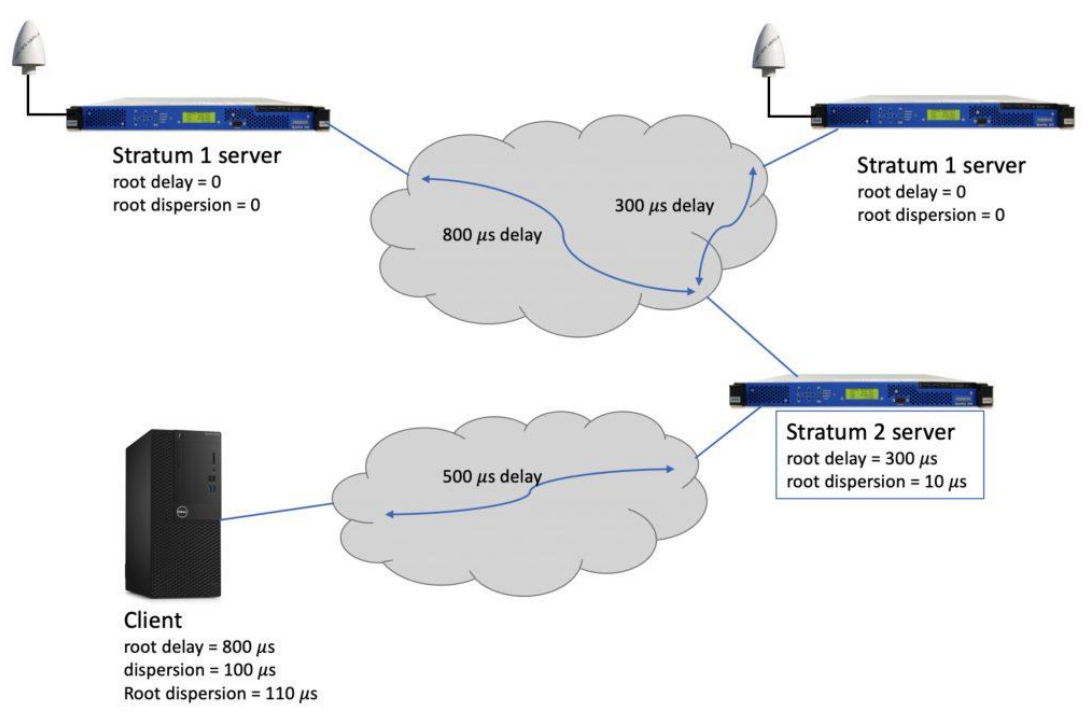
\includegraphics[width=0.7\textwidth]{./images/rootdispersion.png}
    \caption{ Example root dispersion \& root delay }
\end{figure}

\begin{figure}[H]
    \centering
    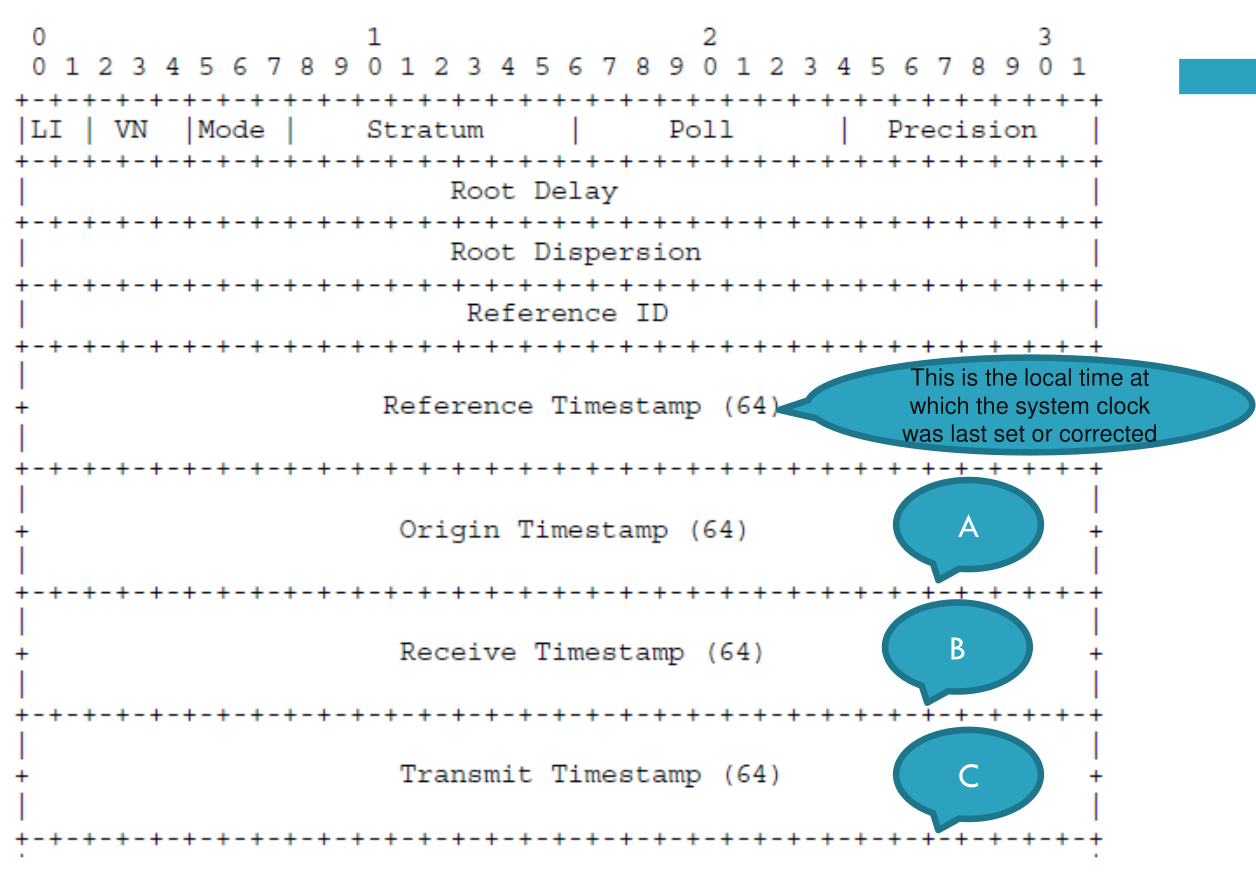
\includegraphics[width=0.7\textwidth]{./images/annotatedntpheader.png}
    \caption{ Annotated NTP protocol header }
\end{figure}

A \textbf{reference ID (refid)} is a 32-bit code (4 ASCII bytes) identifying the particular server or reference clock, e.g.,:
\begin{itemize}
    \item   \verb|GPS|: Global Positioning System;
    \item   \verb|GAL|: Galileo Positioning System;
    \item   \verb|PPS|: Generic Pulse-Per-Second;
    \item   \verb|DCF|: LF Radio DCF77 Mainflingen, DE 77.5 kHz;
    \item   \verb|WWV|: HF Radio WWV Fort Collins, Colorado;
    \item   \verb|GOOG|: unofficial Google refid used by Google NTP servers as \verb|time4.google.com|.
\end{itemize}

\begin{figure}[H]
    \centering
    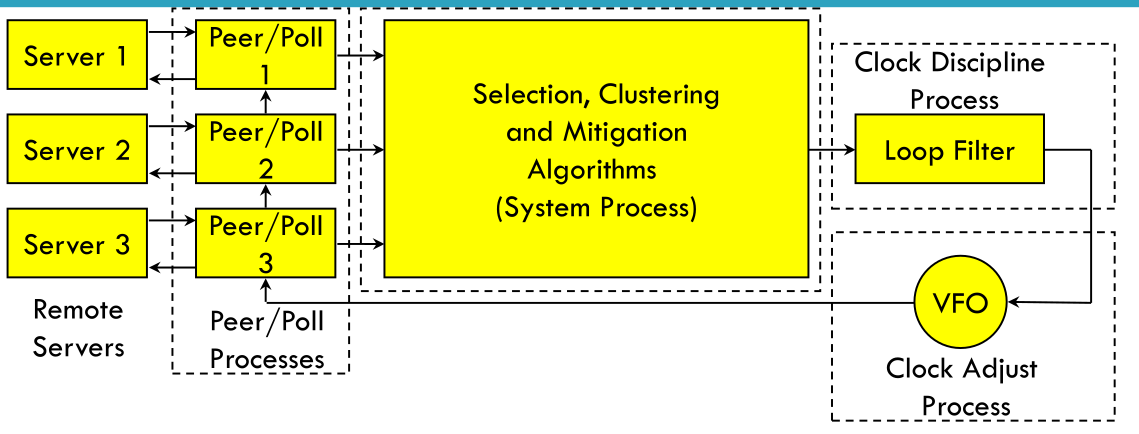
\includegraphics[width=0.7\textwidth]{./images/ntparchitecuraloverview.png}
    \caption{ NTP architectural overview }
\end{figure}

An NTP client synchronises with multiple stratum servers.
It uses a range of algorithms to deal with variable \& asymmetric non-deterministic network delays and to determine its most likely offset, thereby running a series of processes:
\begin{itemize}
    \item   The peer process runs when a packet is received;
    \item   The poll process sends packets at intervals determined by the clock discipline process \& remote server;
    \item   The system process runs when a new update is received;
    \item   The clock discipline process implements clock time adjustments;
    \item   The clock adjust process implements periodic clock frequency (VFO) adjustments.
\end{itemize}

For each stratum there is a \textbf{poll process} that sends NTP packets at intervals ranging from 8 seconds to 36 hours.
The corresponding \textbf{peer processes} receive NTP packets and, after performing some packet sanity tests, $T1$ – $T4$ are determined / extracted.
The NTP daemon calculates offset \& delay as seen before.
The time series of offset \& delay values calculated by multiple peer processes are processed by a sequence of algorithms, thus eliminating servers with long RTD or servers that show ``strange'' offsets which, for example, are often the result of network asymmetries.

\subsubsection{Mitigation Algorithms}
The \textbf{clock filter algorithm} uses a sliding window of eight samples for each stratum server and picks out the sample with the least expected error, i.e., it chooses the sample with the minimum RTD.
It is effective at removing spikes resulting from intermittent network congestions.

\begin{figure}[H]
    \centering
    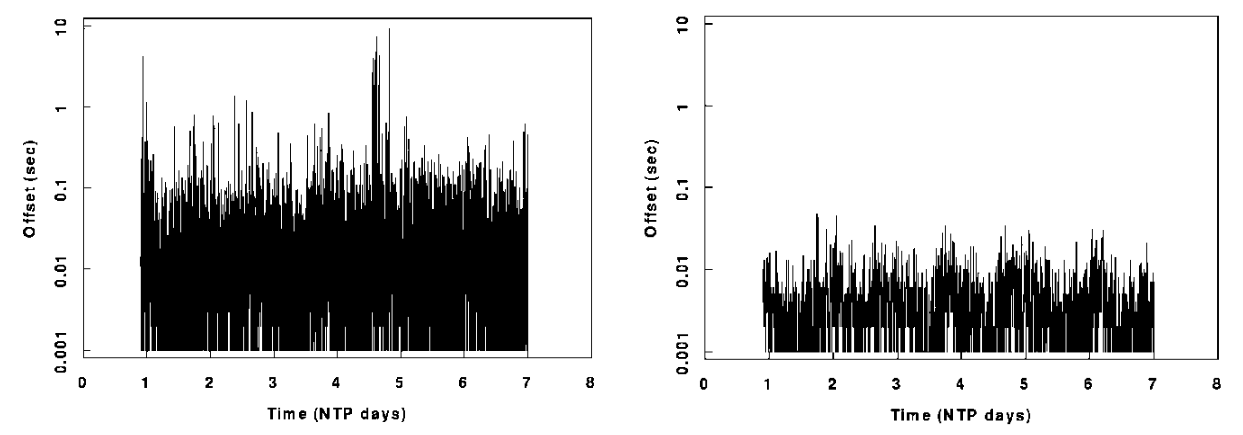
\includegraphics[width=0.7\textwidth]{./images/clockfilteralg.png}
    \caption{ Clock filter algorithm before and after }
\end{figure}

\begin{figure}[H]
    \centering
    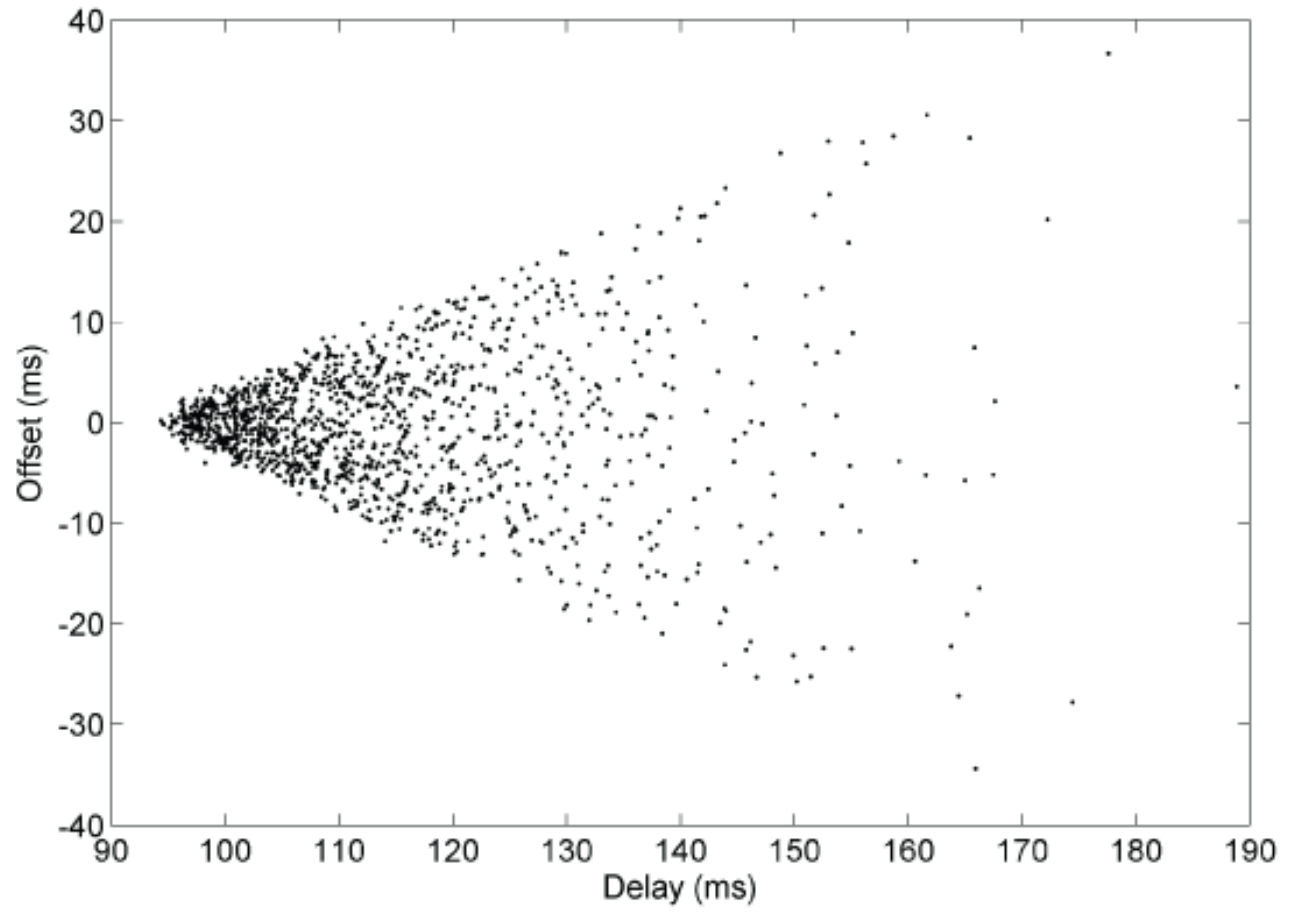
\includegraphics[width=0.7\textwidth]{./images/clockfilteralgmotivation.png}
    \caption{ 
        The wedge scattergram plots sample points of offset versus delay (RTD) collected over a 24-hour period by a client clock communicating with a single stratum server.
        For this experiment, the client clock is externally synced to the stratum server, so the offset should be zero;
        however, as the (network) round trip delay increases, the offset variability increases, resulting in increasingly larger offset errors.
        Therefore, the best samples are those at the lowest delay.
        This is taken into account by the clock filter algorithm.
    }
\end{figure}

The \textbf{intersection algorithm} selects a subset of peers (i.e., stratum servers) and identifies truechimers \& truetickers based on the intersection of confidence (offset) intervals (i.e., min/max offsets of a clock over $x$ readings determines its invterval).

\begin{figure}[H]
    \centering
    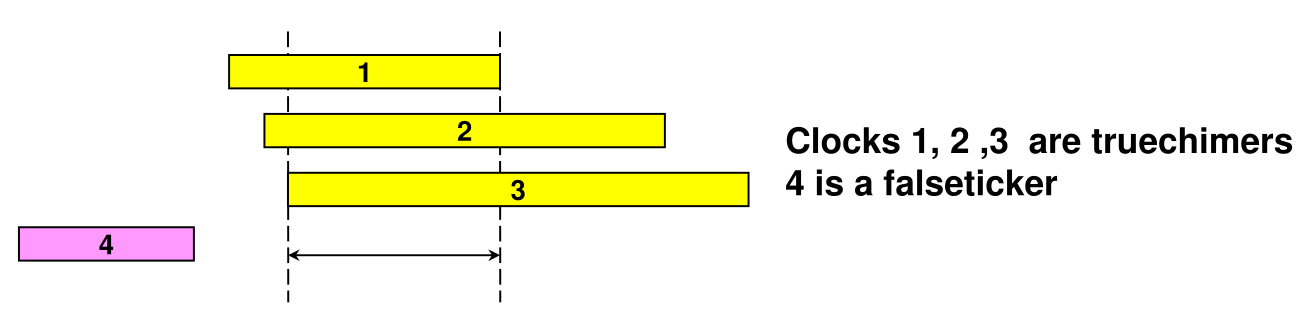
\includegraphics[width=0.7\textwidth]{./images/intersectional.png}
    \caption{ Plot range of offsets calculated by each peer with 1, 2, \& 3 overlapping}
\end{figure}

\textbf{Marzullo's algorithm} is an agreement protocol for estimating accurate time from a number of noisy time sources by intersecting offset intervals; if some intervals don't intersect, it considers the intersection of the majority of intervals.
It eliminates false tickers.
\\\\
The \textbf{clock cluster algorithm} processes the truechimers returned by the clock intersection algorithm.
It produces a list of survivors by eliminating truechimers that have a comparably large root delay \& root dispersion.
Finally, the \textbf{clock combining algorithm} averages the time offsets of survivors using their root dispersions as a weight, i.e., survivors with a small root dispersion have a higher weight.
\\\\
The \textbf{combining algorithm} provides a final offset, so the client clock can be adjusted.
The UNIX Clock Model provides the kernel variable \verb|tickadj| which amortises the required change gradually by making adjustments every tick e.g., every 10 milliseconds.






\end{document}
